Instructions on how to compile and run the project are available in the \texttt{README.md} file in the root of the repository. A brief description of the code structure and implemented functionalities will be presented.

\subsection{Folder structure}
The root directory of the repository contains the following folders:
\begin{itemize}
    \item \texttt{gmsh} contains the \texttt{.geo} files required for \texttt{gmsh} to generate meshes that describe the problem. These files consists in a list of instructions for \texttt{gmsh} to generate the mesh, such as the size the domain, the shape of the domain, the tag of the boundary conditions, etc.
    
    \item \texttt{include} contains the header files for the C++ code, containing declarations of functions and classes, definitions of template functions and type aliases. Most of the comments regarding the functionalities of the code are in the header files.
    
    \item \texttt{scripts} contains shell scripts for generating meshes with different factors or as standalone files and a simple Python script for generating a plot of the drag and lift coefficients, along with the Reynolds number, as a function of the time index. This plot is mainly used to verify that the program is working correctly, by comparing the results to the expected physical behavior of the system.
    
    \item \texttt{src} contains the source files for the C++ code. The \texttt{main.cpp} file contains the \texttt{main()} function, which is the entry point of the program, that reads the user arguments and boots the relative problem.

    \item \texttt{results} is an initially empty folder, which will be filled with output files during execution of the program. Output files are written in the \texttt{.vtk} format, which can be read by \texttt{ParaView} to generate visualizations of the solution. A \texttt{.csv} file is also written, containing the drag and lift coefficients, along with the Reynolds number, as a function of the time index.
    
\end{itemize}

\subsection{Class hierarchy}
The \texttt{NavierStokes<dim>} class template is the main class of the project, which implements the finite element solver. Since we implemented problems with different physical dimensions, the class is templated on the dimension of the problem, which can be either 2 or 3. More classes inherit from it, namely \texttt{Cylinder<dim>}, \texttt{Step} and \texttt{EthierSteinman}. The first one implements the flow past a cylinder problem, while the other two are used for debugging purposes.

\begin{figure}[ht]
\centering

\begin{tikzpicture}
    \umlsimpleclass[x = 4]{NavierStokes$<$dim$>$}{}{}
    \umlsimpleclass[x = 8.5]{BlockPrecondition}{}{}

    \umlsimpleclass[x=2, y=-2]{Cylinder$<$dim$>$}{}{}
    
    \umlsimpleclass[y=-4]{Cylinder2D}{}{}
    \umlsimpleclass[x=3, y=-4]{Cylinder3D}{}{}
    \umlsimpleclass[x=6, y=-4]{Step}{}{}
    \umlsimpleclass[x=9, y=-4]{EthierSteinman}{}{}
    \umlinherit{Cylinder2D}{Cylinder$<$dim$>$}
    \umlinherit{Cylinder3D}{Cylinder$<$dim$>$}
    \umlinherit{Cylinder$<$dim$>$}{NavierStokes$<$dim$>$}
    \umlinherit{Step}{NavierStokes$<$dim$>$}
    \umlinherit{EthierSteinman}{NavierStokes$<$dim$>$}
    \umluniassoc{NavierStokes$<$dim$>$}{BlockPrecondition}
\end{tikzpicture}
\caption{Class relationships}
\label{fig:uml}
\end{figure}

The UML in Figure \ref{fig:uml} shows the relationship between the major classes in the project. The abstract class template \texttt{Navier-Stokes<dim>} implements the usual methods \texttt{setup()}, \texttt{assemble()}, \texttt{solve()} and \texttt{output()} of a finite element solver, each implemented in a separate file. It does not however give an implementation of the initial conditions, boundary functions and kinematic viscosity. Three classes or class templates inherit from it, implementing specific problems:
\begin{itemize}
    \item \texttt{Cylinder<dim>}: This abstract class template is used to provide a common interface for the 2D and 3D flow past a cylinder problems, which are implemented in \texttt{Cylinder2D} and \texttt{Cylinder3D} respectively. Those two classes inherit from \texttt{Cylinder<dim>} instead of using template specialization, as using template specialization would have implied implementing some methods twice.
    \item \texttt{Step}: This class represents a modified version of the problem presented in laboratory 9, which uses the Navier-Stokes equations instead of the Stokes equations. It was used for debugging purposes.
    \item \texttt{EthierSteiman}: This class represents the Ethier-Steinman problem, which will be described in Section \ref{sec:correctness}.
\end{itemize}

Two more elements are worthy of mention: \texttt{BlockPrecondition}, which gives a common interface for the preconditioners for the problem, and \texttt{SolverOptions}, which is a struct containing all parameters used by the linear solver, e.g. tolerance, preconditioner type and maximum number of iterations. Four concrete preconditioners inherit from \texttt{BlockPrecondition} and are described in Section \ref{sec:preconditioners}.

To reduce compile times, allow for compiling with multiple threads, reduce merging issues and improve overall readability and maintenability, each major code functionality is implemented in a separate file. The code was developed starting from laboratory code and then modified to add all the needed functionalities.

\subsection{Mesh generation}
Meshes are generated through the \texttt{gmsh} software, using the \texttt{.geo} files in the \texttt{gmsh} folder. The meshes are generated by running a variety of possible scripts in the \texttt{scripts} folder. To choose the size of finite elements, some bash scripts are provided, which generate meshes with different factors, through the \texttt{-clmax} flag, which is normally used to force the maximum possible diameter of the finite elements. All finite elements that compose the final mesh are simplex finite elements.

Within the \texttt{gmsh} folder, the following files are available:
\begin{itemize}
    \item \texttt{2d-flow.geo} generates a mesh for the 2D flow past a circle problem.
    \item \texttt{3d-flow.geo} generates a mesh for the 3D flow past a cylinder problem.
    \item \texttt{cube-inside-cube.geo} generates a cube with a smaller cube hole inside it, as a simple exercise to learn how to use \texttt{gmsh}.
    \item \texttt{cube.geo} generates a simple cube mesh for the Ethier-Steinman problem.
    \item \texttt{square-inside-square.geo} generates a square with a smaller square hole inside it, as a simple exercise to learn how to use \texttt{gmsh}.
    \item \texttt{uncentered-cube.geo} a variant of \texttt{cube.geo}, which is not centered at the origin, for debugging purposes.
\end{itemize}